\chapter{Lecture Notes}

\section{05.09.24 - Meassurements}

\subsection{Agenda}
The agenda of this lecture is:
\begin{highlight}
    \begin{itemize}
        \item Monitoring a food process – why?
        \subitem * Variability of a process
        \subitem * Type of variations
        \item Characterization of a process by measuring
        \item Classification of process analyzers/sensors
        \item Correlations between measurements
    \end{itemize}
\end{highlight}


\section{05.09.24 - ISO 22000:2018 - A food safety management system standard}


\textbf{Management} is the way in which an organization manages the inter-related parts of its business in order to achieve its objectives.
There were given a link which can be used to get more information:
https://www.iso.org/management-system-standards.html
(5/9/2018)

\textbf{Standard} (= scheme), this describes the set of rules/requirements on which the system of an organization are based…

Here are some examples of Food Safety Management System Standards:
\begin{highlight}
    \begin{itemize}
        \item BRC Global standard – Food
        \item IFS
        \item SQF
        \item ISO 22000
        \item FSSC 22000
        \item For more examples, see QM-textbook, pp. 7-12
    \end{itemize}
\end{highlight}

\subsection{Deming Circle}
The Deming Circle, also known as the PDCA Cycle (Plan-Do-Check-Act), is a continuous improvement model developed by W. Edwards Deming. It consists of four key steps:

\begin{highlight}
    \begin{itemize}
        \item \textbf{Plan} - Identify an opportunity and plan for change.
        \item \textb{Do} - Implement the change on a small scale.
        \item \textbf{Check} - Use data to analyze the results of the change and determine whether it made a difference.
        \item \textbf{Act} - If the change was successful, implement it on a wider scale and continuously assess your results. If the change did not work, begin the cycle again.
    \end{itemize}
\end{highlight}

The PDCA cycle promotes ongoing evaluation and refinement, leading to gradual, sustained improvement in processes or products. This is meant to be a continuous cycle, with each iteration building on the last and can be depicted in \ref{fig:demingcircle}.

\begin{figure}
    \centering
    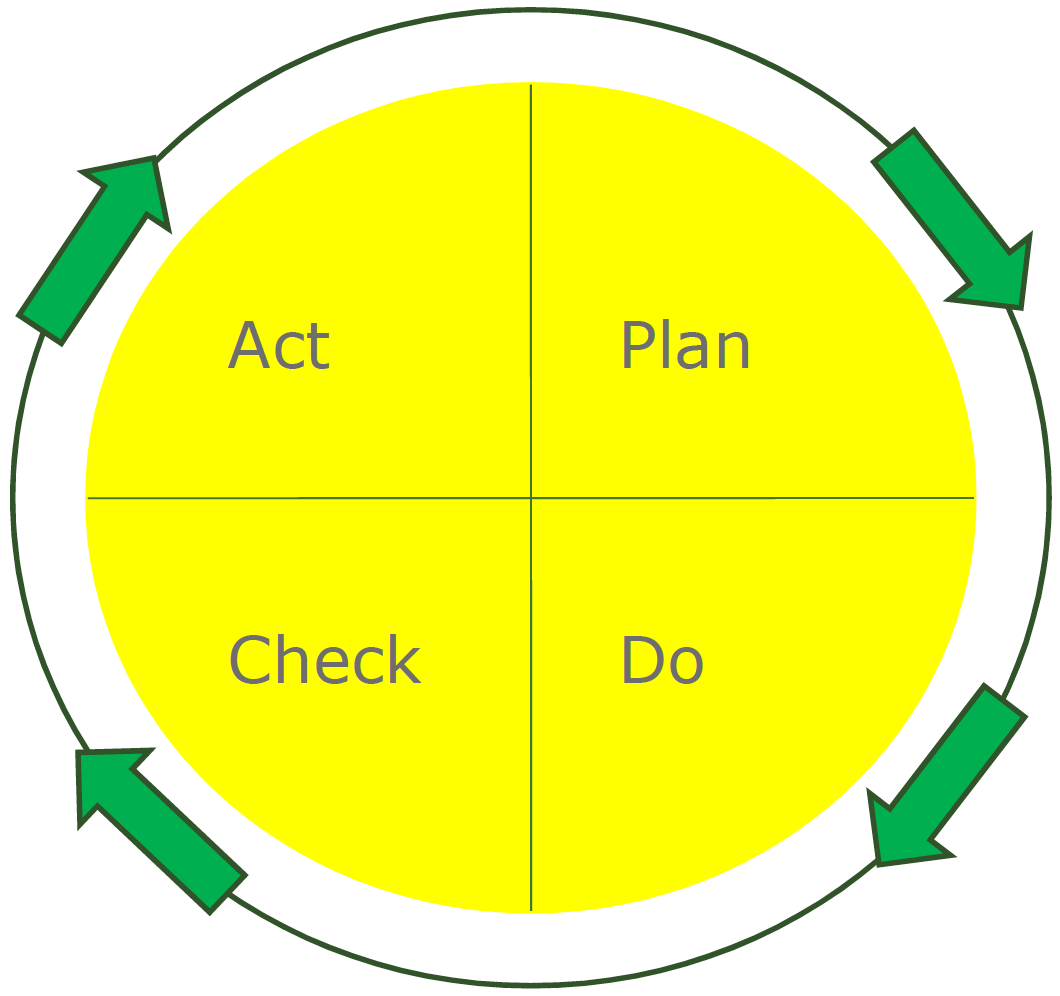
\includegraphics[width=0.5\textwidth]{Figures/DemingCircle.png}
    \caption{A picture of the circular thought behind the Deming Circle}
    \label{fig:demingcircle}
\end{figure}

A more thorough illustration of the four steps can be seen from the following 

\begin{figure}
    \centering
    \includegraphics[width=0.5\textwidth]{Figures/ThroughDC.png}
    \caption{A thorough illustration of the Plan-Do-Check-Act cycle}
    \label{fig:ThoroughDC}
\end{figure}



\subsection{ISO 22000}
Here are three keypoints of the ISO 22000:

\begin{highlight}
    \begin{itemize}
        \item It combines the prerequisite and operational prerequisite
        programmes (i.e. GMP) and HACCP requirements of Codex
        Alimentarius and quality management requirements of ISO 9000
        \item It reduces confusion about Food Safety Management System
        Standard requirements, since it defines the elements of key
        standards required by leading retailer chains in a single standard
        and defines the Codex HACCP system as the ”standard within the
        standard” to be used
        \item however, the standard is generic, i.e. organizations/companies have to think themselves!
    \end{itemize}
\end{highlight}

There are 10 chapters in the ISO 22000 standard, chapter 4-10 are the main chapters. The first three chapters are the introduction and the scope of the standard. Thus chapters 4-10 are the main chapters of the requirements of the standard.

\begin{highlight}
    \begin{itemize}
        \item Chapter 1: Scope
        \item Chapter 2: Normative references
        \item Chapter 3: Terms and definitions
        \item \textbf{Chapter 4: Context of the organization}
        \item \textbf{Chapter 5: Leadership}
        \item \textbf{Chapter 6: Planning}
        \item \textbf{Chapter 7: Support}
        \item \textbf{Chapter 8: Operation}
        \item \textbf{Chapter 9: Performance evaluation}
        \item \textbf{Chapter 10: Improvement}
    \end{itemize}
\end{highlight}





\section{05.09.24 - HACCP - step 9: monitoring procedures}